

% Modeling with graphs
\begin{exer}[Muddy City]
\label{exer_muddy_city}
    There is a famous children's puzzle called "The Muddy City''.
        \begin{quote}
            Once upon a time there was a city that had no roads.  Getting around the city was particularly difficult after rainstorms because the ground became very muddy-- cars got stuck in the mud and people got their boots dirty.  The mayor of the city decided that some of the streets must be paved, but he didn't want to spend more money than necessary because the city also wanted to build a swimming pool.  The mayor therefore specified two conditions.
                \begin{enumerate}
                    \item Enough streets must be paved so that it is possible for everyone to travel from their house to anyone else's house only along paved roads, and
                    \item The paving should cost as little as possible.
                \end{enumerate}
                [\Cref{fig_muddy_city}] shows the layout of the city. The number of paving stones between each house represents the cost of paving that route.
                Source: Computer Science Unplugged
            \end{quote}
    What's the best route?

    \begin{figure}[ht]
         \centering
         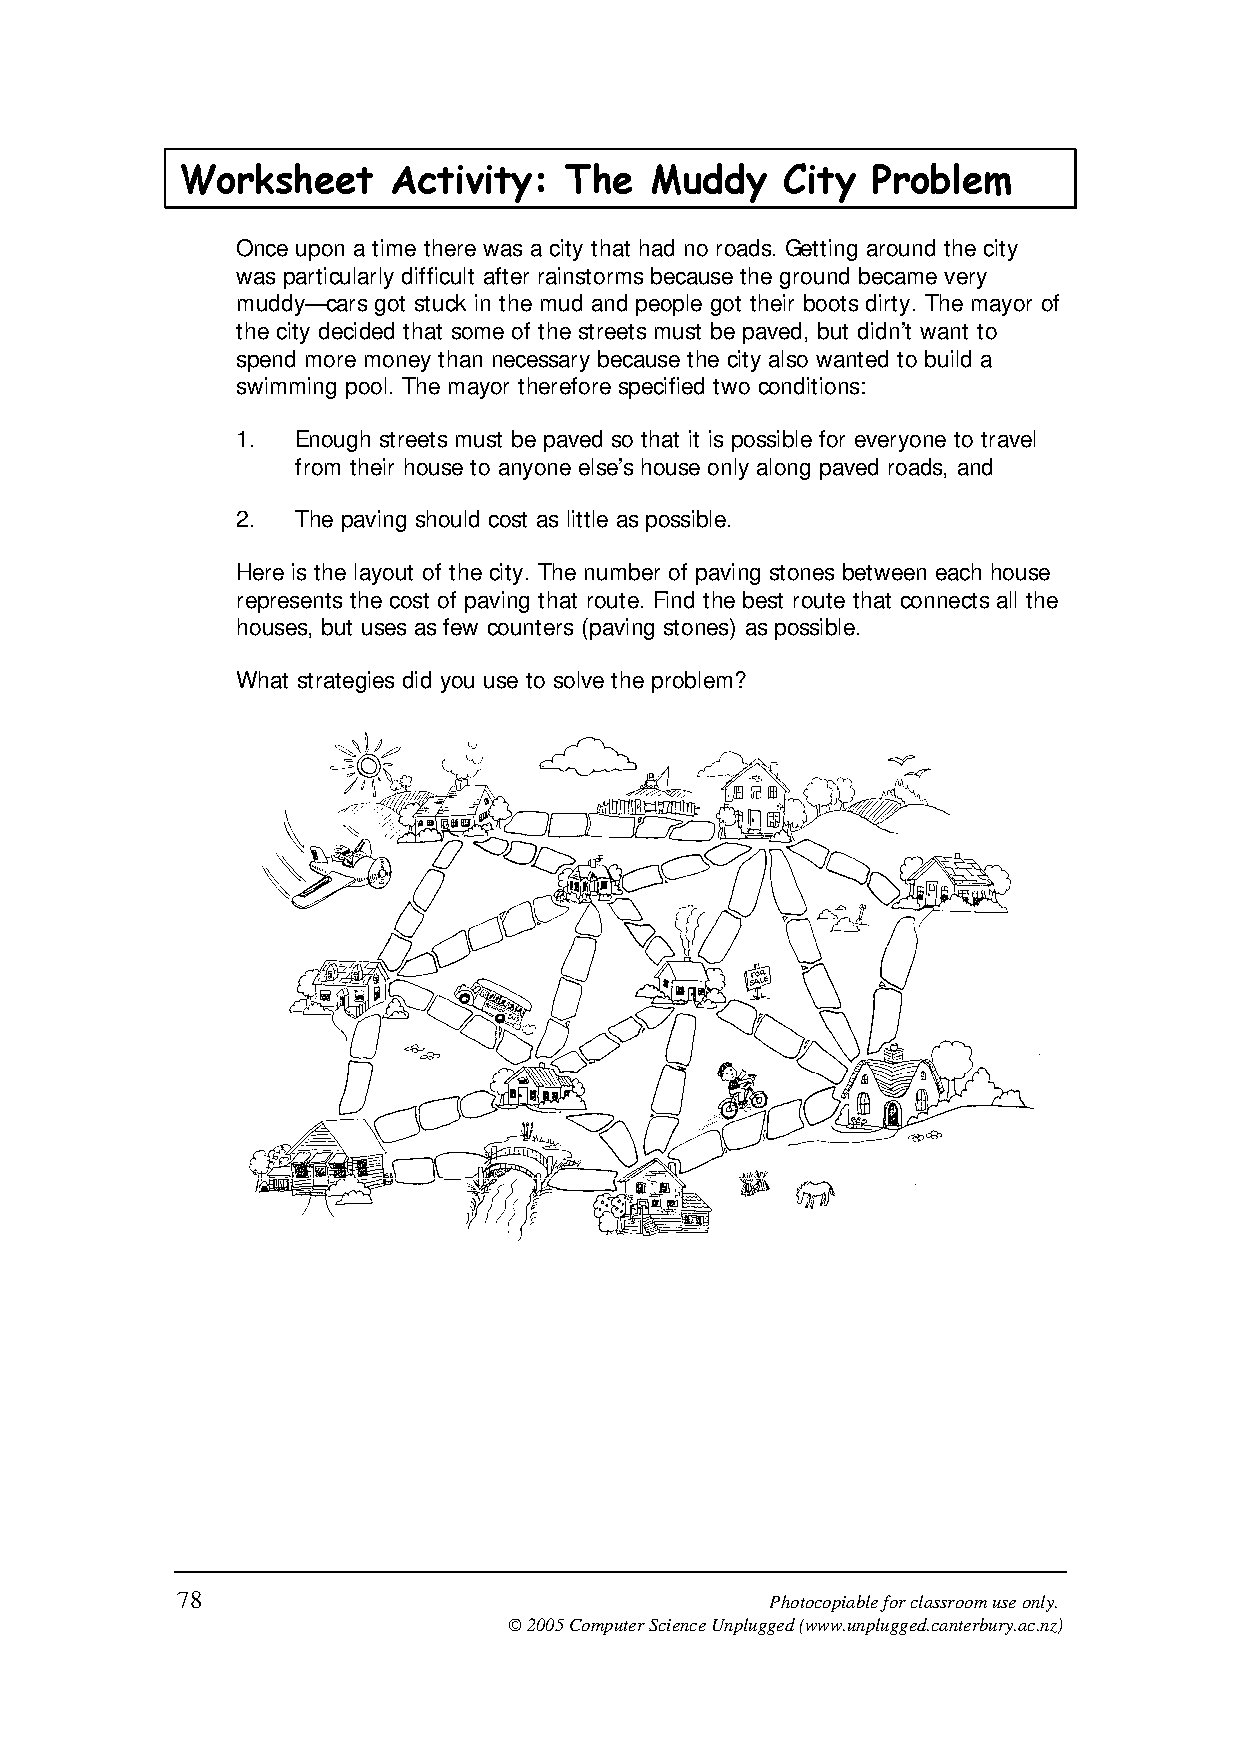
\includegraphics{Images/MuddyCity.pdf}
         \caption{The Muddy City (source:Computer Science Unplugged)}
         \label{fig_muddy_city}
     \end{figure}

    \begin{exerpart}
    \item Draw a graph to represent the Muddy City.  Label each edge with a number representing the cost to pave that route.
    \item Restate the question in terms of the graph.
    \item Then answer the question.  \emph{You do not need to justify that your answer is minimal.}
    \end{exerpart}
\end{exer}

% Modeling with graphs
\begin{exer}[Traveling Salesperson]
SU FIX OR DELETE??
What is the \textbf{traveling salesperson problem}?  Either do an Internet search and describe the problem, or play the Traveling Salesman (using the link on Moodle) and tell me you did that.
\end{exer}